\section{Nash equilibrium, best response, weak dominance, price of anarchy}

\Que{What is a NE}
\Ans[Nash equilibrium ]{is what is played if believes of both players match.}
\Spec{A \textbf{belief} of player $i$ is a possible profile of other player's strategy.

A \textbf{best strategy} is the response of a rational player to a believe. i.e. strategy $s_i \in S_i$ is a BS to moves \m{(s_1,...,s_{i-1},s_{i+1},...,s_n)} if \mat{(s_1,...,s_{i-1},\textcolor{red}{s_i},s_{i+1},...,s_n) \geq (s_1,...,s_{i-1},\textcolor{blue}{s'_{i}},s_{i+1},...,s_n)\\\fa \textcolor{blue}{s'_{i}} \in S_i}}

\Que{Consider NE \m{(s_1,...,s_n)}. Suppose player $i$ replaces the
current strategy $s_i$ with \m{s'_i}. Can this still be a NE?}
\Ans[No.]{ In Nash equilibrium no player can improve his payoff unilaterally.}

\Que{If a strategy is ruled out by IESDS, can it be a NE?}
\Ans[Yes.]{ A joint strategy \m{(s^*_1,...,s^*_n)} in which everyone plays a dominant strategy is a Nash equilibrium.}

\Que{Compute the PoA for the Prisoner’s dilemma using \mat{C(s) = -\sum_j u_j(s)}}
\Ans[]{
\begin{table}[!ht]
    \centering
    \begin{tabular}{cc||c|c}
        \multicolumn{4}{c}{Player B}\\
        \multirow{3}*{\rotatebox{90}{Player A}}
        &    & M     & F     \\ \cline{2-4}
        &M   & -1,-1 & -9,0  \\ \cline{2-4}
        &F   & 0,-9  & -6,-6 \\
    \end{tabular}
    \caption{Prisoners' dilemma}
\end{table}

Worst (and, in this case, unique) NE: MM. Best Pareto: MF or FM. \mat{PoA = \frac{-[-(-1)+(-1)]}{-[(0)+(-6)]} = \frac{2}{6} = \frac{1}{3}}}
\Spec{The price of anarchy (PoA) is the ratio between the social costs in the worst NE $s^*$ and in the best Pareto efficient strategy (i.e.,
social optimum).\mat{PoA = \frac{C (s^{*})}{min_s~C(s)}}}

\Que{Solve this hw.
\begin{figure}[!ht]
    \centering
    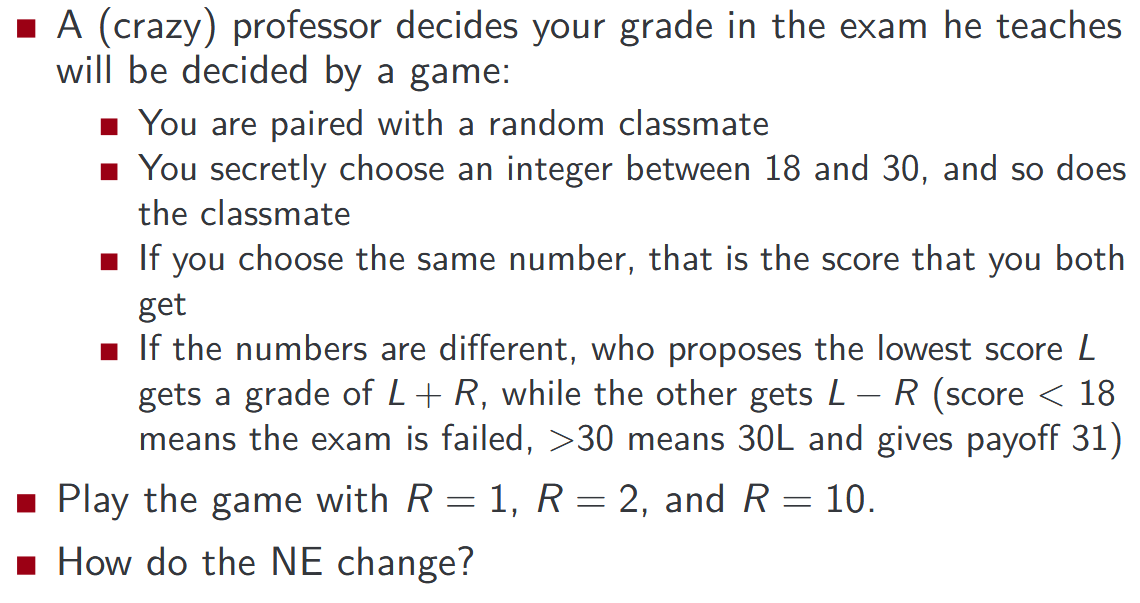
\includegraphics[width=0.5\linewidth]{hw1.png}
\end{figure}
}

\Ans[]{For a generic R
\begin{table}[!ht]
    \centering
    \begin{tabular}{cc|c|c|c|c|c}
        \multicolumn{1}{c}{} & \multicolumn{6}{c}{Player B}\\
        \multirow{6}*{\rotatebox{90}{Player A}}
         & & \textbf{18} & \textbf{19} & \textbf{\dots} & \textbf{29} & \textbf{30}\\ \cline{2-7}
         & \textbf{18} & 18,18 & 18+R,0 & \dots & 18+R,0 & 18+R,0\\ \cline{2-7}
         & \textbf{19} & 0,18+R & 19,19 & \dots & 19+R,21-R & 19+R,19-R\\ \cline{2-7}
         & \textbf{\dots} & \dots & \dots & $\ddots$ & \dots & \dots\\ \cline{2-7}
         & \textbf{29} & 0,18+R & 19-R,19+R & \dots & 29,29 & 29-R,29+R\\ \cline{2-7}
         & \textbf{30} & 0,18+R & 19-R,19+R & \dots & 29-R,29+R & 30,30\\
    \end{tabular}
    \caption{HW1: Strange exam}
\end{table}
\FloatBarrier
For $R = 1$ all couples with same grades are Nash equilibria.

For $R > 1$ the only NE is a Pareto-dominated strategy (i.e., 18,18).
}